\chapter{Twitter Multilayer Ego Networks}
\label{cap:ExpSetup}

In this chapter we define the Twitter multilayer ego network model used in this dissertation and we describe how we collect the dataset used in the experiments. In section \ref{sec:MEN} we have the formal definition of Twitter multilayer ego networks. Section \ref{sec:dataset} describes the procedures for collecting the dataset. In sections \ref{sec:dataset_follow_network} and \ref{sec:dataset_retweets_network} are the formal definitions of how we model the layers of the multilayer ego networks from the collected data.

%%%%%%%%%%%%%%%%%%%%%%%%%%%%%%%%%%%%%%%%%%%%%%%%%%%%%%%%
%%%%%%%%%%%%%%%%%%%%%%%%%%%%%%%%%%%%%%%%%%%%%%%%%%%%%%%%


\section{Definition of Twitter Multilayer Ego Networks}
\label{sec:MEN}
Given a Twitter user $e$, to whom we refer  as {\em ego}, we define the {\em multilayer ego network} $\mathcal{G}_e$ of $e$ 
as a  family of directed graphs  $\mathcal{G}_e=\{G_e^{\alpha};  \alpha \; \in\{1, \cdots m\} \}$. Each  graph  $G_e^{\alpha}$ is  a {\em layer} of $\mathcal{G}_e$ and is associated to a  Twitter interaction  of type $\alpha$.  $G_e^{\alpha}$ is defined as the pair $G_e^\alpha = (\{e\} \cup A_e^{\alpha}, E_e^{\alpha})$.  
Set $\{e\} \cup A^\alpha_e$ is the vertex set of graph $G_e^\alpha$.  $A^{\alpha}$ is the set of  all Twitter users that $e$ has interacted with at least once by interaction of  type $\alpha$. We refer to $A_e^{\alpha}$ as the  {\em alter set of $e$ regarding interaction of type} $\alpha$, or simply as the {\em alter set of} $e$ when the type of interaction is implicit in the context. Set $E_e^{\alpha} =  \{(v_i,v_j) | v_i,v_j \in \{e\} \cup A_e^\alpha: v_i \neq v_j\}$ is the set of directed edges or ordered pairs of the form $(v_i,v_j)$, meaning that user $v_i$ has interacted with user $v_j$ at least once by the interaction of type $\alpha$. 


According to the above definition, a multilayer ego network for a user $e$ has the following characteristics: a) a user $a$ is an alter of $e$ in layer $\alpha$ ($a \in A^{\alpha}_e$), only if $e$ interacted directly with $a$ by an $\alpha$ interaction, i.e., an edge $(e,a)$
must exists in $E_e^{\alpha}$; b) there may  be an edge  $(a_1,a_2)$ (an {\em alter-alter} edge) in $E_e^{\alpha}$ as long as $e$ has interacted with both $a_1$ and $a_2$ by interactions of type $\alpha$ (i.e., $a_1,a_2 \in A_e^{\alpha}$) and $a_1$  has also interacted with  $a_2$ by an interaction of type $\alpha$; c) there may be an edge $(a_1,e)$ (an {\em alter-ego} edge) in $E_e^{\alpha}$ which implies that the  ego $e$ and the alter $a_1$ have both interacted with each other by interaction $\alpha$; d) a same user $a$ may be an alter in as many layers of an ego $e$, as the number of distinct interaction types $e$ has used to interact with $a$. 
 
%Notice that according to the above definition, a multilayer ego-network for a user $e$ has the following characteristics:

%\begin{itemize}
%\item The set of vertices forming a layer is composed only by the ego $e$ herself  and  by the one-step neighbors of $e$ in Twitter according to interaction $\alpha$. That is, we include as the alter set of $e$ only those Twitter users
%that the ego has interacted directly with  by interaction of type $\alpha$. 
%\item An edge $(a_1,a_2)$ such that $a_1 \neq e$ and $a_2\neq e$ pertains to    $E_e^{\alpha}$ if only the pair of edges $(e, a_1)$ and $(e, a_2)$   also pertain  to  $E_e^{\alpha}$. In other words, edge $(a_1,a_2)$ means that $a_1$ has also interacted with $a_2$ by means of interaction of type $\alpha$,  but this edge exists in $E_e^{\alpha}$ only if both vertices are alters of $e$.
%\item   A same alter $a_1$ may take part in more than one layer of an ego $e$. For instance, if $e$ interacted with $a_1$ by means of interactions of types $\alpha_1$ and $\alpha_2$, we have that $a_1$ takes part in both alter set $A_e^{\alpha_1}$ of layer $G_e^{\alpha_1}$ and in alter set $A_e^{\alpha_2}$ of layer $G_e^{\alpha_2}$ .
%\end{itemize}
One may think of  a great number of layers for a multilayer ego network derived from the Twitter OSN, by considering different types of  interactions between pairs of Twitter users. However, in this work, we are interested  in interaction types derived from the four most common  operations  in Twitter:   {\em follow}, {\em retweet}, {\em like} and {\em mention}. The follow operation allows a user $e$ to inform Twitter that $e$ wants  to follow a specific user $a$. This means that $e$ will start receiving in her timeline every tweet authored by or propagated by $a$ via a retweet operation. The mention operation allows a  user $e$ to send a tweet directly to another user $a$. In this case, the tweet works like a message sent by $e$ to $a$. The retweet operation is applied by a user $e$ to a tweet $t$. The effect of the retweet is that $t$ is propagated to all users that follow $e$.  Finally, the like operation is also applied by a user $e$ to a tweet $t$ and simply marks $t$ as a tweet that $e$ liked to receive. 
 
The above four operations in Twitter imply in interactions among users. The follow and the mention are  operations one user perform over another since a user  uses these operations to, respectively,  establish  a communication channel with  or  send a message to  another user. The retweet and like operations are, on the contrary,  operations over a tweet and not directly between users. However, both represent the fact that a user found interesting a piece of text (tweet) authored by another user. In this sense, both are considered  interactions between the receiver and the  writer of the tweet. Thus, from this point on, we refer to follow, mention, like and retweet as  direct interactions between two Twitter users. 
 
\begin{figure}[htb]
	\centering
	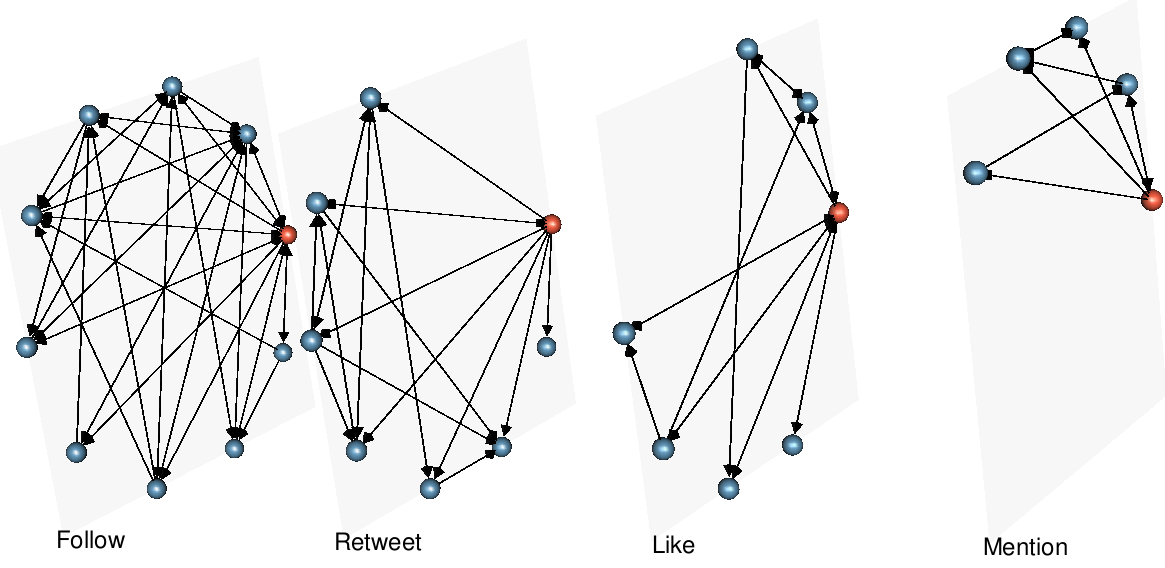
\includegraphics[width=1\textwidth]{fig/multilayer/layers_oneLine.png}
	\caption{Example of a multilayer ego network in Twitter. Ego {\em e} highlighted in red.}
	\label{fig:ex_multilayer}
\end{figure}
 
In this way, for a user $e$,  we can derive four different interaction layers or graphs in Twitter: $G_e^f$, $G_e^m$, $G_e^r$ and  $G_e^l$, where the letter in the superscript of each graph represents   the initial of the corresponding interaction. Each of these graphs are built as described in the first paragraph of this section, by substituting $\alpha$ for {\em follow, mention, retweet} and {\em like} interactions, respectively. Together these four graphs form a multilayer ego network of user $e$, represented as $\mathcal{G}_e=\{G_e^f, G_e^m, G_e^r, G_e^l \}$. Fig. \ref{fig:ex_multilayer} presents an hypothetical example of a multilayer ego network for an ego $e$. 




\section{Dataset} \label{sec:dataset}

We started collecting data with an initial set of users formed by the 100 users who were the last to write a tweet related to any of the ten Twitter trend topics in January, 14, 2017. We adopted a {\em snowball}\footnote{Sampling technique where the data set is formed from initial elements that meet the search criteria, called seeds, and the set grows from these.} strategy to derive a large set of users from which we selected our final sample of users (egos) for whom we obtained the multilayer ego networks.  

Since the layers of the ego networks correspond to interactions in Twitter, we opt to not use Twitter interactions to drive the harvest of users in order to avoid  bias towards any layer type. Thus, we opted to use Twitter lists in the process of expanding the set of users. Also, the choice of using list during the process of obtaining the egos was taken because we wanted to investigated if lists could be uses as ground truth for community detection in each layer for a given ego, as we explain in \ref{sec:QuestionTwitterLists}. 

We first collected a set of {\em possible egos} $P$. During the harvesting process to obtain $P$, we adopted the following expansion criterion: {\em a user would be included in $P$  only if she has subscribed or owned at least one Twitter list with at least five members}. Only eleven of the 100 initial users satisfied this criterion and they were initially inserted in set $P$. 
Starting from the seed set in $P$ our harvest method adopted a breadth-first search where it picked one user $u$ among users already in $P$ and collected the other users in the lists where $u$ was involved. Only the users in the lists that satisfied the expansion criterion defined above were inserted in $P$,  and the process continued by picking another user in $P$ not considered yet. We stopped the harvest process when $P$ contained  a total of 10,000  possible egos.

Only 3,983 of the 10,000 users had public data and they formed the final collected set. From this set, we randomly chose 500 users to form our final ego set $\mathcal{E}$. We limited the number of egos to 500 due to the cost of obtaining, modeling and analyzing all layers for more egos. 

Once the set of egos $\mathcal{E}$ has been collected, we obtained for each ego $e \in \mathcal{E}$ the four layers: $G_e^{f}$, $G_e^{r}$,  $G_e^{l}$ and $G_e^{m}$. Both the ego set $\mathcal{E}$ and the graphs composing the multilayer ego network of users in $\mathcal{E}$ were collected using the Twitter REST API\footnote{https://developer.twitter.com/en/docs/developer-utilities/usage-api/overview.html}. 

The four layers for each ego in $\mathcal{E}$ are defined in \ref{sec:MEN}, however there are some limitations in Twitter API and also some characteristics of Twitter that imposed some restrictions on the number of alters and, consequently, on the number of edges we used to form each layer. In what follows we comment on the difficulties found in collecting alters  and the resulting limitations in the number o alters in each layer.


%%%%%%%%%%%%%%%%%%%%%%%%%%%%%%%%%%%%%%%%%%%%%%%%%%%%%%%%
%%%%%%%%%%%%%%%%%%%%%%%%%%%%%%%%%%%%%%%%%%%%%%%%%%%%%%%%


\section{The \texorpdfstring{$G_e^f$}{Gef} Layer}
%\section{The $G_e^f$ Layer}
\label{sec:dataset_follow_network}

For almost all egos $e$ in  $\mathcal{E}$ we collected all the users that $e$ follows in Twitter (i.e $e$'s followees) to form the alter set $A_e^f$ of $e$.  However, for approximately 15\% of the egos in $\mathcal{E}$, we collected up to 5,000 of their followees. We imposed this limit on the number of followees collected because it would be prohibitive to obtain the whole follow layer for these egos. This is  because the Twitter API limits the number of requests to collect the followees to only 15 requests every 15 minutes and for each followee we would also need to collect its followees in oder to obtain the edges of the follow layer for each ego. Thus the time to collect the complete follow layer would be huge for those egos with more the 5,000 followees.

Once we collected the alter set $A_e^f$ for an ego $e$, we obtained de edge set $E_e^f$ for $G_e^f$. We started by  creating an edge from $e$ to each of her alters. Next, for each alter in $A_e^f$ we obtained its followees and for every followee $b$ of $a$, such that $b \in  \{e\} \cap A_e^f$ we inserted  a direct edge $(a,b)$ in $E_e^f$. 
 


%Once this limitation happens only to few egos in our 500 ego set it is not an important burden in our analysis. For each alter we also collected their followees only to determine the links among alters and $e$.


%%%%%%%%%%%%%%%%%%%%%%%%%%%%%%%%%%%%%%%%%%%%%%%%%%%%%%%%
%%%%%%%%%%%%%%%%%%%%%%%%%%%%%%%%%%%%%%%%%%%%%%%%%%%%%%%%


\section{The \texorpdfstring{$G_e^r$}{Ger}, \texorpdfstring{$G_e^l$}{Gel} and \texorpdfstring{$G_e^m$}{Gem} Layers}
%\section{The $G_e^r$, $G_e^l$  an $G_e^m$ Layers}
\label{sec:dataset_retweets_network}
The Twitter API does not allow for direct requesting the retweets, likes or mentions made by  a user (ego) $e$. It is necessary to collect $e$'s timeline and to inspect all tweets in it to determine which of them were retweeted, liked  or a mention by  $e$. The alter sets $A_e^r$ and $A_e^l$ are composed of the authors of the tweets rewetted and liked by $e$, respectively. The alter set $A_e^m$ is composed of users to whom $e$ sent a mention-tweet.

The timeline of $e$ must be inspected in order to derive these alter sets. However, the Twitter API limits the number of tweets that can be collected in a user timeline to 3,200 tweets.  Thus, the sizes of  the alter sets $A_e^r$, $A_e^l$ and $A_e^m$ are limited to 3,200 users. In practice,  not all of the tweets in a timeline are rewetted, liked or are mentions, thus the sizes of these alters sets tend to have much less than 3,200 alters.

After collecting  the alter set for the four layers, we obtained the edge set for each of them. In each layer, we first create edges between the ego $e$ and each of her alters. Next, for each alter $a$ in a layer, we access $a$'s timeline and for each tweet that $a$ interacted with, we obtain the user $b$  which is the author of the tweet or is mentioned in the tweet. If $b \in \{e\}\cap A_e^f$, we create and edge from $a$ to $b$ in the edge set of the corresponding layer.

%The first line of Tables \ref{tab:numVertices} and \ref{tab:numEdges}  show information about the number of vertices and the number of edges in the 500 $G_e^f$ obtained. 
